\documentclass[a4paper,12pt]{article}
\usepackage{czech}
\usepackage[utf8]{inputenc}
\usepackage{a4wide}
\usepackage[dvipdfm]{graphicx}
\usepackage{graphics}
\usepackage{indentfirst}
\usepackage{fancyhdr}
\usepackage{setspace}
\usepackage{amsmath}
\usepackage{amssymb}
\usepackage{epsfig}

%%\usepackage{nopageno}
%%\usepackage{txfonts}
\usepackage[usenames]{color}
\renewcommand{\d}{\mbox{d}}

\begin{document}
\section{Úkol}
\begin{enumerate}
    \item Proveďte energetickou kalibraci $\alpha$-spektrometru a určete jeho rozlišení.
    \item Určete absolutní aktivitu kalibračního radioizotopu $^{241}$Am.
    \item Změřte závislost ionizační ztráty $\alpha$-částic ve vzduchu při normálním 
    tlaku -d$T$/dx= $f(t)$. Srovnejte tuto závislost se závislotí získanou pomocí empirické formule 
    pro dolet $\alpha$-častic ve vzduchu za normálních podmínek.
    \item Určete energie $\alpha$-částic vzletujících ze vzorku obsahující izotop $^{239}$Pu a příměs 
    izotopu $^{238}$Pu a porovnejte je s tabelovými hodnotami. Stanovne relativní zastoupení izotopu 
    $^{238}$Pu ve vzorku s přesností lepší než 10 \%, jsou-li T$_{1/2}$($^{238}$Pu)=81.71 yr a 
    T$_{1/2}$($^{239}$Pu)=$24.13\cdot10^3$ yr.
\end{enumerate}

\section{Teoretický úvod}
\subsection{$\alpha$-záření}
$\alpha$-záření je typ radioaktivního záření, které je tovřené kladně nabytými heliovými jádry. 
Pochází zejména z rozpadu těžkch prvků, jako je Am a Pu.

\subsection{Rozlišení spektrometru}
Rozlišení spektrometru udává jeho svhopnost rozlišit dvě různé energetické hodnoty. 
Podrobnější informace jsou v \cite{text}. Jeho hodnota je dána vztahem
\begin{eqnarray}
\Gamma=2\sigma\sqrt{2\ln 2}
\label{gamma}
\end{eqnarray}

\subsection{Aktivita}
Aktivita zářiče je dána vztahem
\begin{eqnarray}
A=\frac{\d N}{\d t}.
\end{eqnarray}
Pokud předpokládáme, že se aktivita vzorku po celou dobu měření nemění, můžeme tento vztrah zjednodušit na
\begin{eqnarray}
A=\frac{\Delta A}{\Delta t}.
\end{eqnarray}
Tento předpoklad je dobře splněn, pokud je doba měření výrazně nižší než poločas rozpadu, což je jak u 
Am, tak i Pu splněno dostatečně.

\subsection{Braggova křivka}
Braggova křivka je definována předpisem
\begin{eqnarray}
h(x)=-\frac{\d T}{\d x}
\label{bragg}
\end{eqnarray}

\subsection{Poměr izotopů}
Poměr izotopů zastoupených ve vzorku získáme jednoduše za pomoci upravení rozpadové rovnice
\begin{eqnarray}
P=\frac{X_1}{X_2}\frac{1-e^{\frac{t\ln 2}{T_{2,1/2}}}}{\frac{t\ln 2}{T_{1,1/2}}},
\label{p}
\end{eqnarray}
kde $X_i$ je počet interakcí s detektorem naměřených pro určitý izotop za dobu $t$, přičem izotom 
má poločas rozpadu $T_{i,1/2}$


\section{Měření}
\subsection{Kalibrace}
Za pomoci známé energie $\alpha$-částic radioizotopu Am jsme provedli kalibraci spektrometru. Naměřené hosnoty jsou v prvním řádku tabulky \ref{mer}. 
Z hodnoty pološířky a vztahu \ref{gamma} jsem stanovil rozlišení spektrometru na
\begin{eqnarray}
\Gamma = 0.3 \mbox{keV}.
\end{eqnarray}

\subsection{Aktivaita vzorku}
Plocha histogramu odpovídá počtu interakcí na detektoru za dobu měření. Naše měření trvalo 500 sekund. Detektor měl tvar kruhu o průměru 
\begin{eqnarray}
d=1.123\pm0.005 \mbox{cm}
\end{eqnarray}
a byl ve vzdálenosti
\begin{eqnarray}
x=3.0\pm0.1 \mbox{cm}
\end{eqnarray}
od vzorku. Vzorek považujeme za bodový a detektor můžeme aproximovat kulovou úsečí. Pro absolutní aktivitu pak získáme vztah
\begin{eqnarray}
A=\frac{N}{t}=4\pi\frac{N_m}{\Omega_dt}=16x\frac{N_m}{d^2t},
\end{eqnarray}
což dá po dosazení naměřených hodnot
\begin{eqnarray}
A=367000\pm1000 \mbox{s}^{-1}
\end{eqnarray}

\subsection{Závislost ionizačních ztrát}
Pro provedení kalibrace jsme provedli měření pro různé hodnoty tlaku v komoře. Naměřené hodnoty 
jsou v tabulce \ref{mer}

\begin{table}
$$
\begin{array}{|c|c|c|c|c|c|c|}
\hline
p/\mbox{bar}&E\mbox{keV}&\mbox{FHHM}&S&\mbox{backg}&\mbox{NET C/S}& \mbox{ERR}\\ \hline
0.0&5485.73&28.23&48132&162&96.264&0.46\\ \hline
0.1&5241.00&39.71&47925&240&95.850&0.46\\ \hline
0.2&4990.52&52.86&48282&127&96.564&0.46\\ \hline
0.3&4733.02&69.41&48231&174&96.462&0.46\\ \hline
0.4&4470.75&84.84&48002&97&96.001&0.46\\ \hline
0.5&4198.63&101.11&48135&139&96.270&0.46\\ \hline
0.6&3917.96&117.67&48437&99&96.874&0.46\\ \hline
0.7&3633.86&136.26&48435&135&96.870&0.46\\ \hline
0.8&3309.94&156.69&48424&162&96.848&0.46\\ \hline
0.9&2953.28&185.95&48197&131&96.394&0.46\\ \hline
0.97&2644.14&211.98&48122&217&96.244&0.46\\ \hline
\end{array}
$$
\caption{Měření energi $\alpha$-částic pro různé hodnoty tlaku}
\label{mer}
\end{table}
Z těchto hodnot následně dopočítáme ionizační ztráty. Hodnoty jsou v tabulce \ref{iz}.

\begin{table}
$$
\begin{array}{|c|c|}
\hline
p/\mbox{bar}& \Delta T/\mbox{keV} \\ \hline
0.0&0.0\pm0.4\\ \hline
0.1&244.7\pm0.5\\ \hline
0.2&495.2\pm0.5\\ \hline
0.3&752.7\pm0.6\\ \hline
0.4&1015.0\pm0.7\\ \hline
0.5&1287.1\pm0.8\\ \hline
0.6&1567.8\pm0.8\\ \hline
0.7&1851.9\pm0.9\\ \hline
0.8&2175.8\pm1.0\\ \hline
0.9&2532.4\pm1.2\\ \hline
0.97&2841.6\pm1.3\\ \hline
\end{array}
$$
\caption{Ionizační ztráty $\alpha$-částic v závislosti na tlaku}
\label{iz}
\end{table}

\begin{figure}
\begin{center}
% GNUPLOT: LaTeX picture with Postscript
\begingroup
  \makeatletter
  \providecommand\color[2][]{%
    \GenericError{(gnuplot) \space\space\space\@spaces}{%
      Package color not loaded in conjunction with
      terminal option `colourtext'%
    }{See the gnuplot documentation for explanation.%
    }{Either use 'blacktext' in gnuplot or load the package
      color.sty in LaTeX.}%
    \renewcommand\color[2][]{}%
  }%
  \providecommand\includegraphics[2][]{%
    \GenericError{(gnuplot) \space\space\space\@spaces}{%
      Package graphicx or graphics not loaded%
    }{See the gnuplot documentation for explanation.%
    }{The gnuplot epslatex terminal needs graphicx.sty or graphics.sty.}%
    \renewcommand\includegraphics[2][]{}%
  }%
  \providecommand\rotatebox[2]{#2}%
  \@ifundefined{ifGPcolor}{%
    \newif\ifGPcolor
    \GPcolorfalse
  }{}%
  \@ifundefined{ifGPblacktext}{%
    \newif\ifGPblacktext
    \GPblacktexttrue
  }{}%
  % define a \g@addto@macro without @ in the name:
  \let\gplgaddtomacro\g@addto@macro
  % define empty templates for all commands taking text:
  \gdef\gplbacktext{}%
  \gdef\gplfronttext{}%
  \makeatother
  \ifGPblacktext
    % no textcolor at all
    \def\colorrgb#1{}%
    \def\colorgray#1{}%
  \else
    % gray or color?
    \ifGPcolor
      \def\colorrgb#1{\color[rgb]{#1}}%
      \def\colorgray#1{\color[gray]{#1}}%
      \expandafter\def\csname LTw\endcsname{\color{white}}%
      \expandafter\def\csname LTb\endcsname{\color{black}}%
      \expandafter\def\csname LTa\endcsname{\color{black}}%
      \expandafter\def\csname LT0\endcsname{\color[rgb]{1,0,0}}%
      \expandafter\def\csname LT1\endcsname{\color[rgb]{0,1,0}}%
      \expandafter\def\csname LT2\endcsname{\color[rgb]{0,0,1}}%
      \expandafter\def\csname LT3\endcsname{\color[rgb]{1,0,1}}%
      \expandafter\def\csname LT4\endcsname{\color[rgb]{0,1,1}}%
      \expandafter\def\csname LT5\endcsname{\color[rgb]{1,1,0}}%
      \expandafter\def\csname LT6\endcsname{\color[rgb]{0,0,0}}%
      \expandafter\def\csname LT7\endcsname{\color[rgb]{1,0.3,0}}%
      \expandafter\def\csname LT8\endcsname{\color[rgb]{0.5,0.5,0.5}}%
    \else
      % gray
      \def\colorrgb#1{\color{black}}%
      \def\colorgray#1{\color[gray]{#1}}%
      \expandafter\def\csname LTw\endcsname{\color{white}}%
      \expandafter\def\csname LTb\endcsname{\color{black}}%
      \expandafter\def\csname LTa\endcsname{\color{black}}%
      \expandafter\def\csname LT0\endcsname{\color{black}}%
      \expandafter\def\csname LT1\endcsname{\color{black}}%
      \expandafter\def\csname LT2\endcsname{\color{black}}%
      \expandafter\def\csname LT3\endcsname{\color{black}}%
      \expandafter\def\csname LT4\endcsname{\color{black}}%
      \expandafter\def\csname LT5\endcsname{\color{black}}%
      \expandafter\def\csname LT6\endcsname{\color{black}}%
      \expandafter\def\csname LT7\endcsname{\color{black}}%
      \expandafter\def\csname LT8\endcsname{\color{black}}%
    \fi
  \fi
  \setlength{\unitlength}{0.0500bp}%
  \begin{picture}(7200.00,5040.00)%
    \gplgaddtomacro\gplbacktext{%
      \csname LTb\endcsname%
      \put(1210,704){\makebox(0,0)[r]{\strut{} 0}}%
      \put(1210,1382){\makebox(0,0)[r]{\strut{} 500}}%
      \put(1210,2061){\makebox(0,0)[r]{\strut{} 1000}}%
      \put(1210,2739){\makebox(0,0)[r]{\strut{} 1500}}%
      \put(1210,3418){\makebox(0,0)[r]{\strut{} 2000}}%
      \put(1210,4096){\makebox(0,0)[r]{\strut{} 2500}}%
      \put(1210,4775){\makebox(0,0)[r]{\strut{} 3000}}%
      \put(1342,484){\makebox(0,0){\strut{} 0}}%
      \put(2263,484){\makebox(0,0){\strut{} 0.5}}%
      \put(3184,484){\makebox(0,0){\strut{} 1}}%
      \put(4105,484){\makebox(0,0){\strut{} 1.5}}%
      \put(5027,484){\makebox(0,0){\strut{} 2}}%
      \put(5948,484){\makebox(0,0){\strut{} 2.5}}%
      \put(6869,484){\makebox(0,0){\strut{} 3}}%
      \put(308,2739){\rotatebox{-270}{\makebox(0,0){\strut{}$T$/keV}}}%
      \put(4105,154){\makebox(0,0){\strut{}$p$/bar}}%
    }%
    \gplgaddtomacro\gplfronttext{%
      \csname LTb\endcsname%
      \put(3982,4602){\makebox(0,0)[r]{\strut{}fitovaný polynom}}%
      \csname LTb\endcsname%
      \put(3982,4382){\makebox(0,0)[r]{\strut{}naměřená hodnoty}}%
    }%
    \gplbacktext
    \put(0,0){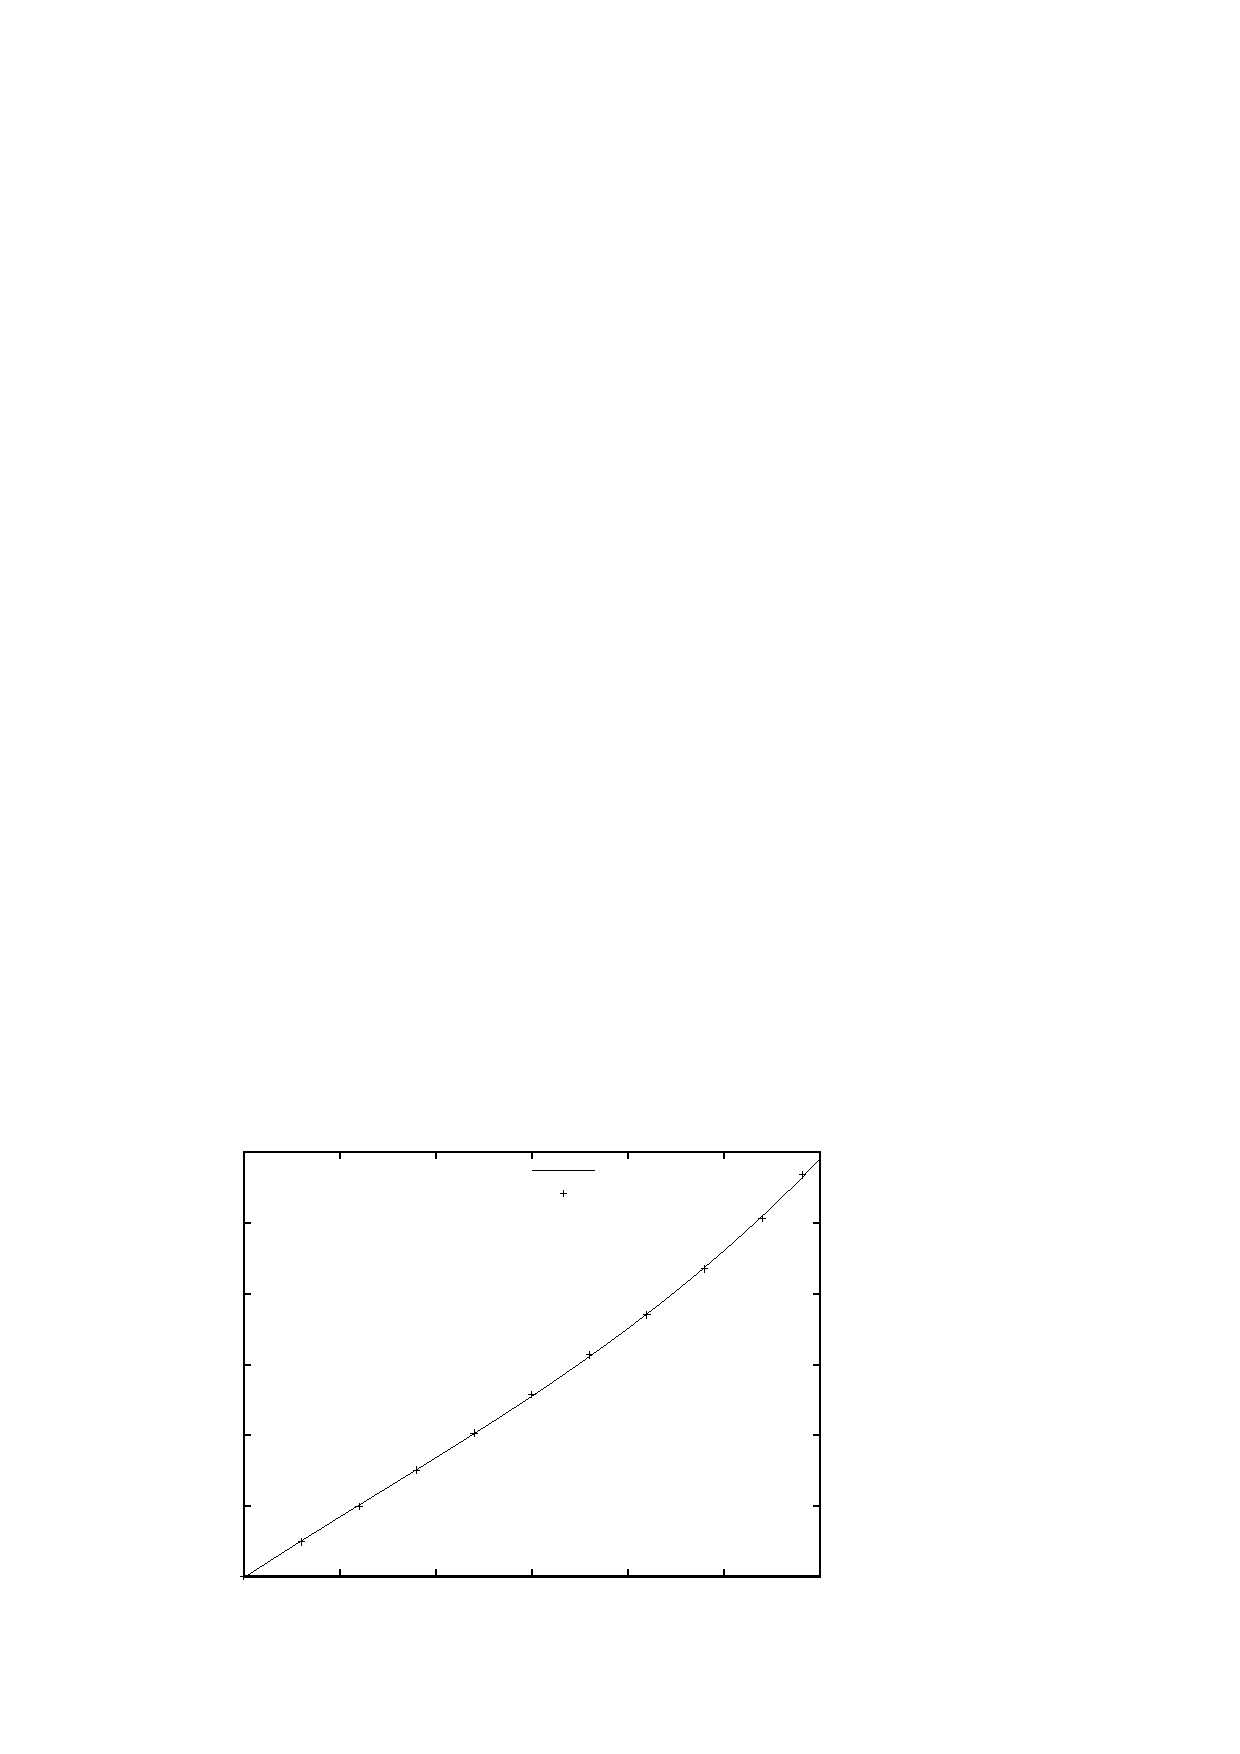
\includegraphics{g}}%
    \gplfronttext
  \end{picture}%
\endgroup
o
\end{center}
\caption{Graf závislosti ionizačních ztrát na tlaku}
\label{g}
\end{figure}



\subsection{Specifické ztráty}
Naměřeným energiím jsem nafitoval polynom s předpisem
\begin{eqnarray}
T(x)=-36.4*x^3+77*x^2-890*x+5494
\end{eqnarray}
Tomuto předpisu odpovídá dle \ref{bragg} Braggova křivka
\begin{eqnarray}
h(x)=109.2*x^2-154*x+890
\end{eqnarray}
Pro názornost je na obrázku \ref{o1}.

\begin{figure}
\begin{center}
% GNUPLOT: LaTeX picture with Postscript
\begingroup
  \makeatletter
  \providecommand\color[2][]{%
    \GenericError{(gnuplot) \space\space\space\@spaces}{%
      Package color not loaded in conjunction with
      terminal option `colourtext'%
    }{See the gnuplot documentation for explanation.%
    }{Either use 'blacktext' in gnuplot or load the package
      color.sty in LaTeX.}%
    \renewcommand\color[2][]{}%
  }%
  \providecommand\includegraphics[2][]{%
    \GenericError{(gnuplot) \space\space\space\@spaces}{%
      Package graphicx or graphics not loaded%
    }{See the gnuplot documentation for explanation.%
    }{The gnuplot epslatex terminal needs graphicx.sty or graphics.sty.}%
    \renewcommand\includegraphics[2][]{}%
  }%
  \providecommand\rotatebox[2]{#2}%
  \@ifundefined{ifGPcolor}{%
    \newif\ifGPcolor
    \GPcolorfalse
  }{}%
  \@ifundefined{ifGPblacktext}{%
    \newif\ifGPblacktext
    \GPblacktexttrue
  }{}%
  % define a \g@addto@macro without @ in the name:
  \let\gplgaddtomacro\g@addto@macro
  % define empty templates for all commands taking text:
  \gdef\gplbacktext{}%
  \gdef\gplfronttext{}%
  \makeatother
  \ifGPblacktext
    % no textcolor at all
    \def\colorrgb#1{}%
    \def\colorgray#1{}%
  \else
    % gray or color?
    \ifGPcolor
      \def\colorrgb#1{\color[rgb]{#1}}%
      \def\colorgray#1{\color[gray]{#1}}%
      \expandafter\def\csname LTw\endcsname{\color{white}}%
      \expandafter\def\csname LTb\endcsname{\color{black}}%
      \expandafter\def\csname LTa\endcsname{\color{black}}%
      \expandafter\def\csname LT0\endcsname{\color[rgb]{1,0,0}}%
      \expandafter\def\csname LT1\endcsname{\color[rgb]{0,1,0}}%
      \expandafter\def\csname LT2\endcsname{\color[rgb]{0,0,1}}%
      \expandafter\def\csname LT3\endcsname{\color[rgb]{1,0,1}}%
      \expandafter\def\csname LT4\endcsname{\color[rgb]{0,1,1}}%
      \expandafter\def\csname LT5\endcsname{\color[rgb]{1,1,0}}%
      \expandafter\def\csname LT6\endcsname{\color[rgb]{0,0,0}}%
      \expandafter\def\csname LT7\endcsname{\color[rgb]{1,0.3,0}}%
      \expandafter\def\csname LT8\endcsname{\color[rgb]{0.5,0.5,0.5}}%
    \else
      % gray
      \def\colorrgb#1{\color{black}}%
      \def\colorgray#1{\color[gray]{#1}}%
      \expandafter\def\csname LTw\endcsname{\color{white}}%
      \expandafter\def\csname LTb\endcsname{\color{black}}%
      \expandafter\def\csname LTa\endcsname{\color{black}}%
      \expandafter\def\csname LT0\endcsname{\color{black}}%
      \expandafter\def\csname LT1\endcsname{\color{black}}%
      \expandafter\def\csname LT2\endcsname{\color{black}}%
      \expandafter\def\csname LT3\endcsname{\color{black}}%
      \expandafter\def\csname LT4\endcsname{\color{black}}%
      \expandafter\def\csname LT5\endcsname{\color{black}}%
      \expandafter\def\csname LT6\endcsname{\color{black}}%
      \expandafter\def\csname LT7\endcsname{\color{black}}%
      \expandafter\def\csname LT8\endcsname{\color{black}}%
    \fi
  \fi
  \setlength{\unitlength}{0.0500bp}%
  \begin{picture}(7200.00,5040.00)%
    \gplgaddtomacro\gplbacktext{%
      \csname LTb\endcsname%
      \put(946,704){\makebox(0,0)[r]{\strut{} 0}}%
      \put(946,1111){\makebox(0,0)[r]{\strut{} 20}}%
      \put(946,1518){\makebox(0,0)[r]{\strut{} 40}}%
      \put(946,1925){\makebox(0,0)[r]{\strut{} 60}}%
      \put(946,2332){\makebox(0,0)[r]{\strut{} 80}}%
      \put(946,2740){\makebox(0,0)[r]{\strut{} 100}}%
      \put(946,3147){\makebox(0,0)[r]{\strut{} 120}}%
      \put(946,3554){\makebox(0,0)[r]{\strut{} 140}}%
      \put(946,3961){\makebox(0,0)[r]{\strut{} 160}}%
      \put(946,4368){\makebox(0,0)[r]{\strut{} 180}}%
      \put(946,4775){\makebox(0,0)[r]{\strut{} 200}}%
      \put(1078,484){\makebox(0,0){\strut{}-30}}%
      \put(2032,484){\makebox(0,0){\strut{}-20}}%
      \put(2986,484){\makebox(0,0){\strut{}-10}}%
      \put(3941,484){\makebox(0,0){\strut{} 0}}%
      \put(4895,484){\makebox(0,0){\strut{} 10}}%
      \put(5849,484){\makebox(0,0){\strut{} 20}}%
      \put(6803,484){\makebox(0,0){\strut{} 30}}%
      \put(176,2739){\rotatebox{-270}{\makebox(0,0){\strut{}$I$/rel. j.}}}%
      \put(3940,154){\makebox(0,0){\strut{}$x$/mm}}%
    }%
    \gplgaddtomacro\gplfronttext{%
    }%
    \gplbacktext
    \put(0,0){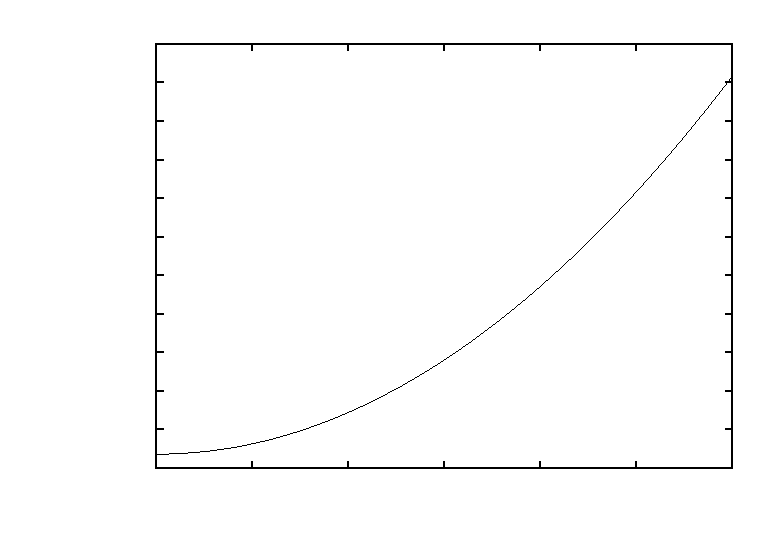
\includegraphics{g1}}%
    \gplfronttext
  \end{picture}%
\endgroup
o
\end{center}
\caption{Bragoova křivka pro měřený vzorek}
\label{o1}
\end{figure}

\subsection{Pu}
Provedl jsem měření pro vzorek ze směsi plutonia izotopů 238 a 239. Pro Jenotlivé píky jsem získal hodnoty uvedené  v tabulce \ref{pu}.

\begin{table}
$$
\begin{array}{|c|c|c|c|c|c|c|}
\hline
&E\mbox{keV}&\mbox{FHHM}&S&\mbox{backg}&\mbox{NET C/S}& \mbox{ERR}\\ \hline
^{239}\mbox{Pu}&5142.42&34.26&106570&321&213.140&0.31\\ \hline
^{238}\mbox{Pu}&5484.98&40.25&917&5&1.834&3.27\\ \hline
\end{array}
$$
\caption{Hodnoty naměřené pro smět Pu izotopů 238 a239}
\label{pu}
\end{table}

Poměr izotopů 238 ku 239 následně získáme po dosazení do vtahu \ref{p}
\begin{eqnarray}
P=29.1 \pm 0.6
\end{eqnarray}

\section{Diskuze}
V celém měření se vyskytovali velmi malé chyby. To především velmi dobrému rozlišení spektrometru. 
Dále se do hodnot v podstatě neprojevovali vnější zdroje, což také přispělo k přesnosti měření. 
Získané honoty odpovídají předpokládaným teoretickým výsledkům.

\section{Závěr}
\noindent
Provedl jsem kalibraci spektrometru. \\
Určil jsem rozlišovací schopnost spektrometru
\begin{eqnarray}
\Gamma=0.3 \mbox{keV}
\end{eqnarray}
Změřil jsem ionizační ztrátu $\alpha$-částic na tlaku. Výsledeky je v tabulce \ref{iz} na obrázku \ref{g}. \\
Stanovil jsem Braggovu křivku, která je na obrázku \ref{o1}. \\
Stanovil jsem poměr izotopů 238 ku 239 v Pu
\begin{eqnarray}
P=29.1\pm 0.6
\end{eqnarray}

\begin{thebibliography}{5}
	\bibitem{text} \textbf{Studijní text na praktikum IV} \\http://physics.mff.cuni.cz/vyuka/zfp/txt\_405.pdf (16. 10. 2012)
    \bibitem{chyba} \emph{J. Englich}: \textbf{Zpracování výsldků fyzikálních měření} \\ LS 1999/2000
\end{thebibliography}

\end{document}
